\documentclass[a4paper,12pt,titlepage]{article}
\usepackage[portuguese]{babel}
\usepackage[utf8]{inputenc}
\usepackage[T1]{fontenc}
\usepackage{mathtools}
\usepackage{amssymb}
\usepackage{amsmath}
\usepackage{algorithm}% http://ctan.org/pkg/algorithms
\usepackage{algpseudocode}% http://ctan.org/pkg/algorithmicx
\usepackage{url}
\usepackage{texdraw}
\usepackage{gnuplottex}
\usepackage{caption}
\usepackage{subcaption}
\usepackage[section]{placeins}
\let\biconditional\leftrightarrow
\begin{document}

\title{Relatório do Trabalho de Conceção e Análise de Algoritmos}
\date{27 de abril 2015}
\author{Francisco Veiga, up201201604@fe.up.pt
 \and João Cabral, up201304395@fe.up.pt
 \and  João Mota, up201303462@fe.up.pt\linebreak
 \and Faculdade de Engenharia da Universidade do Porto}
%\input{./title_page_1.tex}
\maketitle
\tableofcontents
\newpage
\section{Introdução}

No contexto da unidade curricular de Conceção e Análise de Algoritmos, foi solicitada a resolução de um problema relacionado com a distribuição de uma rede de fibra ótica pela rede habitacional de um determinado agregado populacional.

\section{Problemas a abordar} 
Numa primeira fase, é solicitada uma aplicação que receba como dados de entrada um mapa do referido agregado populacional e produza como saída, sob a forma de um grafo, a representação gráfica de uma distribuição ideal da rede de fibra ótica, minimizando o comprimento das ligações utilizadas. Estabelece-se ainda, como restrição adicional, que cada uma das casas cobertas não pode situar-se fora de uma determinada área a ser definida por uma distância máxima à central de onde parte a rede de fibra ótica.
 
Numa segunda fase, é solicitado que a aplicação alargue o raio de ação de cobertura da rede de fibra ótica, procurando abranger uma maior área, sendo contudo necessário que a aplicação seja capaz de detetar áreas onde a cobertura providenciada por uma única central se revele insuficiente e seja capaz de indicar a necessidade de existirem novas centrais de distribuição da rede.
\section{Casos de Utilização}
Está implementada a funcionalidade que, abstraindo uma zona a cobrir com rede de fibra ótica como um grafo onde os nós são casas e as arestas as ligações entre elas, permite calcular qual a distribuição ótima de fibra a utilizar para minimizar a quantidade de cablagem necessária à cobertura completa de uma zona, bem como ao estabelecimento de um limite máximo para esse alcance. É também possível identificar as zonas para as quais será necessário instalar centrais adicionais, por não existir ligação direta com outras zonas.

\newpage
\section{Formalização do problema}

\subsection{1º problema/fase}
\subsubsection*{Inputs}
\begin{itemize}
\item Um grafo  $G= ( V, E ) $ conexo, onde $V$ é o conjunto das casas e $E$ o conjunto das suas ligações e para cada aresta $(u,v)\in E$ temos $w(u,v)$ representando a distância entre as arestas $u$ e $v$ e $d(p)$ como sendo a distância de um caminho $p = \langle v_0,v_1,\ldots , v_k\rangle$\cite[p.~624]{intro_algo};
\item Uma distancia $l:l > 0$;
\item Um vértice $s:s\in V$.
\end{itemize}

\subsubsection*{Outputs}
\begin{itemize}
\item Um grafo $G_T = ( V_T,E_T )$ tal que se verifique a condição\cite[p.~643]{intro_algo}:
$$ \forall v \in V(\delta(s,v) \leq l \biconditional v \in V_T)$$
$$\delta(s,v) = 
\begin{cases}
\min \{d(p): s \leadsto^p v\} & \text{se existe caminho entre s e v}\\
\infty & \text{caso contrário} 
\end{cases}$$
\end{itemize}

\subsubsection*{Função Objetivo}
Seja $$x(u,v) = \begin{cases}	
1 & \text{se a aresta} (u,v) \in E_T\\
0 & \text{caso contrário} 
\end{cases}$$

A função objetivo é\cite{ieor_mst}
$$\min \sum_{(u,v)\in E} w(u,v)x(u,v)$$

com as restrições 
$$\sum_{(u,v)\in E} x(u,v) = |V_T| - 1$$
$$\sum_{(u,v)\in (S,S)} x(u,v) \leq |S| - 1 \quad \forall S \subseteq  V_T$$

\subsection{2º problema/fase}
\subsubsection*{Inputs}
\begin{itemize}
\item Um grafo  $G= ( V, E ) $, desconexo ou não, onde $V$ é o conjunto das casas e $E$ o conjunto das suas ligações e para cada aresta $(u,v)\in E$ temos $w(u,v)$ representando a distância entre as arestas $u$ e $v$ e $d(p)$ como sendo a distância de um caminho $p = \langle v_0,v_1,\ldots , v_k\rangle$\cite[p.~624]{intro_algo};
\end{itemize}

\subsubsection*{Outputs}
\begin{itemize}
\item Um grafo $G_T = ( V_T,E_T )$;
\item Um conjunto de grafos $D \subseteq G_T = \{d(V_D,E_D): \forall d,e \in D(\nexists v \in V_T(v \in d \land v \in e)) \land \nexists d,e\in D(\exists(u,v) \in E_T(u \in d \land v \in e)) \}$
\item Um conjunto $S = \{s : \exists! d \in D(s \in d)\}$.
\end{itemize}

\subsubsection*{Função Objetivo}
Seja $$x(u,v) = \begin{cases}
1 & \text{se a aresta} (u,v) \in E_T\\
0 & \text{caso contrário} 
\end{cases}$$

A função objetivo é\cite{ieor_mst}
$$\min \sum_{(u,v)\in E} w(u,v)x(u,v)$$

com as restrições 
$$\sum_{(u,v)\in E} x(u,v) = |V_T| - 1$$
$$\sum_{(u,v)\in (S,S)} x(u,v) \leq |S| - 1 \quad \forall S \subseteq V_T$$
\linebreak
\linebreak
\linebreak
\linebreak
\section{Soluções implementadas}
\subsection{1º Problema/Fase}
Para a resolução deste problema, recorreu-se a dois algoritmos conhecidos que operam sobre grafos: o algoritmo de \emph{Dijkstra} para cálculo das distâncias mínimas de todos os nós a uma determinada fonte e o algoritmo de \emph{Prim} para cálculo da árvore de expansão mínima do grafo. Para a implementação da fila de prioridades recorreu-se ao \emph{Heap de Fibonacci} da biblioteca \emph{Boost}. 
\subsubsection{Algoritmo de Dijkstra}

\begin{algorithmic}[1]
\Procedure{Dijkstra}{fonte, limite, grafo}
\State $vertices \gets grafo.vertices$
\For{Q $\in$ vértices}
\State $Q.dist \gets \infty$
\State $Q.path \gets NULL$
\EndFor
\State $fonte \gets 0$
\State $FH.push(fonte)$
\While{$FH \neq \varnothing$}
\State $v \gets FH.pop()$
\For{$a \in v.adjacencias$}
\If{$v.dist + w < a.dist$}
	\State $a.dist \gets v.dist + w$
	\State $a.path \gets v$
	\If{$a \notin FH$}
		\State $FH.push(a)$
	\Else
		\State $FH.decreaseKey()$
	\EndIf
\EndIf
\EndFor
\EndWhile
\EndProcedure
\Procedure{Podar grafo}{grafo, limite}
\For{$v \in grafo.vertices$}
\If{$v.dist > limite$}
\State $grafo.removeVertice(v)$
\EndIf
\EndFor
\EndProcedure
\end{algorithmic}

O algoritmo de \emph{Dijkstra} foi artilhado com a possibilidade de remover os nós cuja distância à fonte exceda um determinado limite.

\subsubsection{Algoritmo de Prim}
\begin{algorithmic}[1]
\Procedure{Prim}{grafo}
\State $novoGrafo \gets \varnothing$
\State $vértices \gets grafo.vértices$
\For{Q $\in$ vértices}
\State $Q.key \gets \infty$
\State $Q.path \gets NULL$
\State $Q.visited \gets false$
\EndFor
\State $FH.enqueue(vértices)$
\While{$FH \neq \varnothing$}
\State $v \gets FH.pop()$
\State $novoGrafo \gets path(v, v.path)$
\State $v.visited \gets true$
\For{$a \in v.adj$}
\If{$a.key > weight(v,a)$ AND $d.visited = false $}
\State $a.key \gets weight(v,a)$;
\State $a.path \gets v$
\State $a.decreaseKey()$
\EndIf
\EndFor
\EndWhile
\EndProcedure

\end{algorithmic}


\subsection{2º Problema/Fase}
Para resolver este problema, torna-se necessário identificar conjuntos de subgrafos desconexos. O algoritmo de \emph{Prim} já identifica a árvore de expansão mínima de cada subgrafo desconexo, mas não efetua a identificação dos subgrafos desconexos em si mesmos. Tornou-se portanto necessário adaptar levemente o dito algoritmo. Em concreto, de cada vez que um vértice é removido da fila e não possui um antecessor, o grafo construido até agora é guardado numa fila e começa a ser construído um novo grafo. Fica garantido o facto de não serem abandonados vértices do grafo anterior porque os vértices do próximo grafo são inicializados com uma chave infinita, só sendo retirados da fila quando todo o restante grafo já foi percorrido.

\section{Análise de complexidade}
\subsection[Grafo]{Grafo\footnote{Analisam-se exclusivamente as operações do grafo utilizadas no programa desenvolvido.}}

\subsubsection{Inserção de Vértices}
No contexto da nossa aplicação optamos por utilizar uma implementação \emph{naïve} que se limita a acrescentar o vértice a um vetor de vértices, sem verificar repetição de elementos. Tem uma complexidade $O(1)$.

\subsubsection{Inserção de Arestas}
É necessário percorrer o conjunto de vértices para verificar a existência do destino e da fonte da aresta. Tem portanto uma complexidade $O(V)$.

\subsubsection{Remoção de Vértices}
É necessário percorrer o conjunto de vértices para encontrar o vértice pretendido, e depois novamente para encontrar e apagar todas as arestas que apontam para este vértice. Tem por isso uma complexidade $O(V^2+E)$.


\subsection{Algoritmo de Dijkstra}
Sendo \emph{V} o número de vértices a analisar e \emph{E} o número de arestas, o algoritmo percorre primeiramente toda a lista de vértices para inicializar valores. Esta operação tem complexidade \emph{V}.Acrescenta-se, com complexidade $O(1)$, a fonte à fila de prioridade. De seguida, percorre-se a fila de prioridade, recorrendo à função de extração do menor elemento da fila. Num \emph{heap de Fibonacci} esta operação corre em tempo $log(V)$. Obtém-se assim para este ciclo uma complexidade $Vlog(V)$. Dentro deste ciclo, todas as arestas do grafo acabam por ser analisadas, sendo, quando encontrada uma aresta que constitua um caminho mais favorável, chamada a função DecreaseKey do \emph{heap de Fibonacci}, que corre em tempo constante. Obtém-se assim uma complexidade linear $O(E)$.

Por último e como característica particular do problema em causa, torna-se necessário percorrer novamente a lista de vértices no sentido de remover todos aqueles cuja distância à fonte seja excessiva. Dentro deste ciclo pode ou não ser chamada a função removeVertex, que, na nossa implementação do grafo, tem complexidade $O(V^2+ E)$, ficando este ciclo com complexidade $O(V^3+VE)$. Tem-se assim uma complexidade total $O(V+E+Vlog(V)+V(V^2+E)) = O(E+V(VlogV+V^2+E)$.

\subsection{Algoritmo de Prim}
Este algoritmo tem complexidade semelhante ao algoritmo de Dijkstra no ciclo principal. Contudo, de cada vez que um vértice é retirado da fila de prioridade, o mesmo tem que ser adicionado ao grafo resultante e uma aresta tem que ser adicionada de e para o seu predecessor. Esta operação pode ser feita em tempo linear $O(V)$. Ficamos assim com uma complexidade $O(E+V(V+ logV))=O(E+V^2)$.

\section{Análise Empírica}
Para geração dos grafos a utilizar na análise empírica da performance dos algoritmos, foi utilizado o modelo de \emph{Erdős–Rényi}. Este modelo considera o grafo aleatório $G(n,p)$ como sendo um grafo de $n$ nós em que cada par de nós único tem uma probabilidade $p$ de ser ligado por uma aresta, também ela de peso aleatório. Os algoritmos até agora descritos foram corridos sobre grafos gerados segundo este modelo. Num primeiro momento, o número de nós foi fixado em 200 e fez-se variar a conectividade dos grafos. Posteriormente, fixou-se a probabilidade de cada aresta e fez-se variar o número de arestas. Para que que a aleatoriedade associada ao modelo usado tivesse impacto mínimo na análise, efetuou-se cada teste 10 vezes, calculando depois a média dos tempos necessários. Os gráficos abaixo apresentam um sumário desses resultados.
\newpage
\subsection{Algoritmo de Dijkstra}
\begin{figure}[!h]
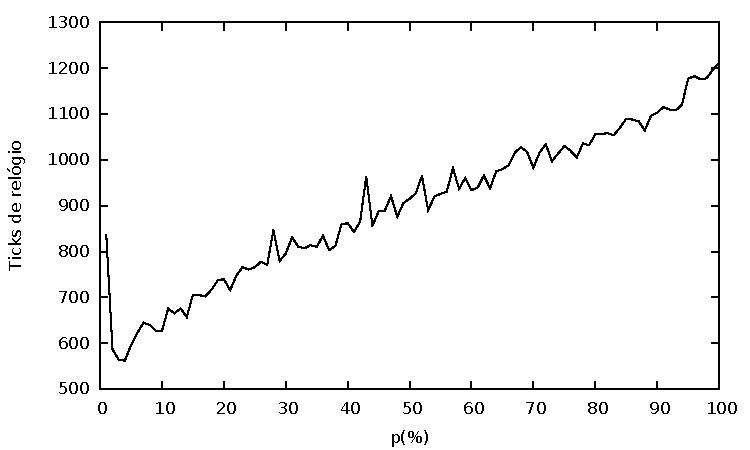
\includegraphics{dijkstra_edges.pdf}
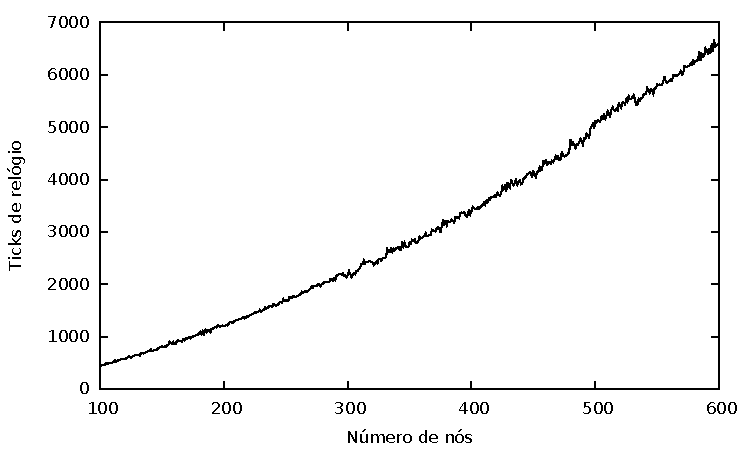
\includegraphics{dijkstra_nodes.pdf}
\caption{Variação da performance do algoritmo de Dijkstra com o número de arestas e vértices.}
\end{figure}

Contrariamente ao que se poderia esperar, o algoritmo parece aumentar o seu tempo de execução de forma aproximadamente linear, quer com o número de arestas, quer com o número de vértices.
\subsection{Algoritmo de Prim}
\begin{figure}[!h]
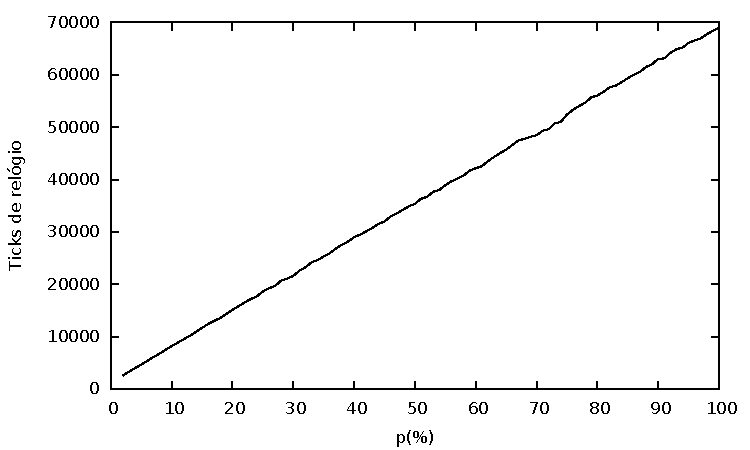
\includegraphics{prim_edges.pdf}
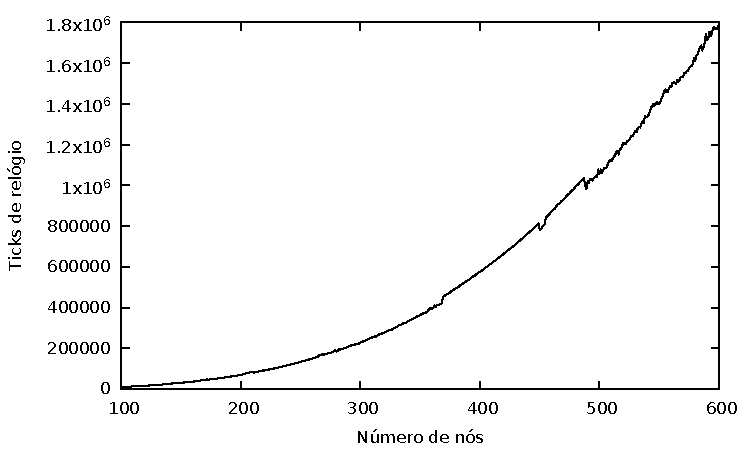
\includegraphics{prim_nodes.pdf}
\caption{Variação da performance do algoritmo de Prim com o número de arestas e vértices.}
\end{figure}
Os resultados confirmam a análise de complexidade efetuada para o algoritmo de Prim implementado. O tempo de execução aumenta linearmente com o número de arestas e quadraticamente com o número de vértices.
\newpage
\section{Considerações sobre a realização do trabalho}
\subsection{Principais dificuldades sentidas}
Sentimos dificuldade em escrever uma especificação detalhada do trabalho, devido a certos aspetos do enunciado que não consideramos estarem suficientemente claros.

Além disso, foi-nos difícil concluir a parte do trabalho respeitante ao \emph{OpenStreetMap}, visto que o programa providenciado para interpretação não funcionou corretamente até uma data muito próxima da entrega.
\subsection{Contribuição dos elementos}
Todos os membros contribuíram para o trabalho, desenvolvendo funcionalidades do programa, bem como colaborando na formalização matemática do problema, na implementação de algoritmos, na descrição da solução e na análise empírica dos tempos de execução.
\begin{description}
\item[Francisco Veiga] Trabalhou no mecanismo de leitura de grafos a partir de um ficheiro de texto, na conceção e compreensão dos algoritmos a usar e nos mecanismos de teste empírico da performance dos mesmos;
\item[João Cabral] Trabalhou na formalização matemática do problema, no algoritmo de Prim e na realização dos testes de performance empíricos e interface com o visualizador de grafos, bem como na elaboração do relatório;
\item[João Mota] Trabalhou no mecanismo de leitura de grafos a partir de um ficheiro de texto, na conceção e compreensão dos algoritmos e implementou o algoritmo de Dijkstra adaptado para remover os vértices que se encontrem fora de um raio especifico. Implementou a totalidade da interface.


\end{description}

\newpage
\bibliographystyle{plain}
\bibliography{cal}


\end{document}
